\begin{frame}
  \frametitle{A math frame}
  
  \begin{theorem}[Pythagoras]
    The square of the hypotenuse of a \alert{right} triangle is equal to the sum of the squares on the other two sides:
    \[
      a^2 + b^2 = c^2.
    \]
  \end{theorem}
  \begin{proof}
    Straightforward.
  \end{proof}
\end{frame}

\begin{frame}{A math frame}{with plotting of math functions}
	
	\begin{definition}[Weibull Random Variable]
		A random variable is said to be \alert{Weibull distributed} with parameters $\delta,\beta$ and $\theta >0$, if its probability density function is given by: \vskip-0.5em
		$$f(t)=\frac{\beta}{\theta} \left ( \frac{t-\delta}{\theta}\right)^{\beta-1} e^{-\left ( \frac{t-\delta}{\theta}\right)^{\beta}}, \quad t \ge 0 $$
		\vskip-0.5em
		The parameters are called: \\ \small
		\qquad $\theta$ --  the scale parameter, $\beta$ --  the shape parameter, $\delta$ --  the location parameter.

	\end{definition}
	\centering%\qquad\qquad\qquad
	\begin{tikzpicture}[font=\footnotesize,
	    declare function={weibullpdf(\x,\delta,\beta,\theta) = (( \x - \delta )/\theta)^(\beta-1) * exp( -((\x - \delta )/\theta)^\beta) *\beta /\theta ;}
		]
	
		\begin{axis}[clip=false, scale = 0.9, font=\scriptsize,
			y post scale = 0.35,
		    axis lines=left,
		    enlargelimits=upper,
		    samples=50,
		    legend entries={$\delta=0 \ \ \beta=1 \quad \ \theta=1$, $\delta=0 \ \ \beta=1.5 \quad \!\!\theta=1$, $\delta=0 \ \ \beta=5 \quad \ \theta=1$},
			xlabel style={at={(axis description cs:0.98,0.05)}, anchor=south},
			xlabel=$x$,  
			ylabel style={at={(axis description cs:0.08,0.8)}, anchor=west},
	    	ylabel=$f(x)$,		    
		]
			\addplot [smooth, very thick,  domain=0:6, kugreen!60!black] {weibullpdf(x,0,1,1)};
			\addplot [smooth, very thick,  domain=0:6, kured] {weibullpdf(x,0,1.5,1)};
			\addplot [smooth, very thick,  domain=0:6, kublue] {weibullpdf(x,0, 5,1)};
		\end{axis}
	\end{tikzpicture}
	

\end{frame}


\begin{frame}
  \frametitle{Environments}
  
  \begin{definition}
    A \textbf{prime number} (or a prime) is a natural number which has exactly two distinct natural number divisors: 1 and itself. 
  \end{definition}
  
  \begin{exampleblock}{Example}
    The first five prime numbers are $2$, $3$, $5$, $7$, and $11$.
  \end{exampleblock}
  
  \begin{alertblock}{Alert block}
    Note that $1$ is not a prime number.
  \end{alertblock}
\end{frame}

\begin{frame}{Using graphics}{with the help of the TikZ library}
	\vskip-0.9em
	\begin{exampleblock}{Exercise}
		Compute $Var[{X}]$ when $X$ represents the dice-rolling experiment using the definitions above.
	\end{exampleblock}

	
	\smallskip
	\qquad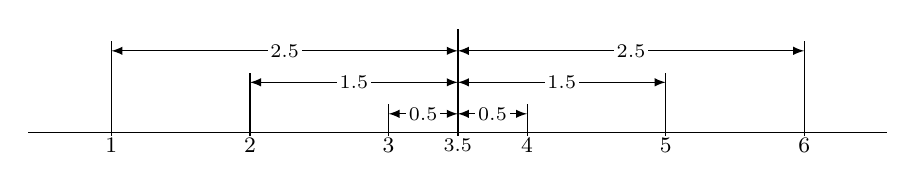
\begin{tikzpicture}[every node/.style={inner sep=1pt,outer sep=0}, xscale=2.2, scale=0.8]
		\draw[thin](0.4, 0) -- (6.6,0);
		\draw[thick] (3.5,-0.05) node[below, font=\scriptsize] {3.5} --++(0,1.7); 

		\foreach \x in {3,4}{ 
				\draw[thin](\x,-0.05) node[below, font=\footnotesize] {\x}  --++(0,0.5); 	
				\draw[thin,latex-latex](3.5,0.3) --node[fill=white, font=\scriptsize]{$0.5$} (\x,0.3); 
		}

		\foreach \x in {2,5}{ 
				\draw[thin](\x,-0.05) node[below, font=\footnotesize] {\x}  --++(0,1); 	
				\draw[thin,latex-latex](3.5,0.8) --node[fill=white, font=\scriptsize]{$1.5$} (\x,0.8); 
		}

		\foreach \x in {1,6}{ 
				\draw[thin](\x,-0.05) node[below, font=\footnotesize] {\x}  --++(0,1.5); 	
				\draw[thin,latex-latex](3.5,1.3) --node[fill=white, font=\scriptsize]{$2.5$} (\x,1.3); 
		}
		
	\end{tikzpicture}
	\smallskip
	\small
	{
	\begin{align*}
		\pause
		Var[{X}] &= E\left [{X-E\left [{X}\right]^2 }\right ] \\
				 & = \frac{1}{6}2.5^2 +  \frac{1}{6}1.5^2 +  \frac{1}{6}0.5^2 +  \frac{1}{6}0.5^2 +  \frac{1}{6}1.5^2 +  \frac{1}{6}2.5^2  = 2.916667\\[8pt]
		\pause
		Var[{X}] &= E\left [{X-E\left [{X}\right ]^2}\right ]  = E\left [{X^2}\right ]-E\left [{X}\right ]^2\\
				 & = \frac{1}{6}(1^2 +  2^2 +  3^2 +  4^2 + 5^2 + 6^2)  - 3.5^2 = 2.916667
	\end{align*}}
	
\end{frame}

\newcommand{\extractHTML}[1]{\extractcolorspecs{#1}{\model}{\mycolor} \convertcolorspec{\model}{\mycolor}{HTML}\printcol \printcol}
\newcommand{\extractRGB}[1]{\extractcolorspecs{#1}{\model}{\mycolor} \convertcolorspec{\model}{\mycolor}{RGB}\printcol \printcol}
\newcommand{\extractCMYK}[1]{\extractcolorspecs{#1}{\model}{\mycolor} \convertcolorspec{\model}{\mycolor}{cmyk}\printcol \printcol}
\newcommand{\colrow}[1]{{\color{#1}#1} & \extractRGB{#1} & \extractCMYK{#1} & \extractHTML{#1}}

\newcommand{\ccft}[3]{
	\usebeamercolor{#1}
	\definecolor{#2}{named}{fg}
	\definecolor{#3}{named}{bg}
}

\ccft{block title}{myblock title fg}{myblock title bg}
\ccft{block body}{myblock body fg}{myblock body bg}
\ccft{block title alerted}{myblock title alerted fg}{myblock title alerted bg}
\ccft{palette secondary}{palette secondary fg}{palette secondary bg}


\begin{frame}{Color definitions}
	\begin{center}
		\vskip-2em\small
		\begin{tabular}{cccc}
			\toprule
			\multicolumn{1}{c|}{\textsc{Color}} &
			\multicolumn{1}{c}{\textsc{RGB}} &
			\multicolumn{1}{c}{\textsc{CMYK}} &
			\multicolumn{1}{c}{\textsc{HTML}}\\
			\midrule 
			\colrow{structure.fg}\\
			\colrow{structure.bg}\\
			\colrow{alerted text.fg}\\
			\colrow{example text.fg}\\
			\colrow{normal text.fg}\\
			\colrow{myblock title fg}\\
			\colrow{myblock title bg}\\
			\colrow{myblock body fg}\\
			\colrow{myblock body bg}\\
			\colrow{myblock title alerted fg}\\
			\colrow{myblock title alerted bg}\\
			\colrow{palette secondary fg}\\
			\colrow{palette secondary bg}\\
			\bottomrule
		\end{tabular}
	\end{center}

\end{frame} 